\chapter{Business-Cycle Properties}\label{chp:bcpr}
\hypertarget{cycles}{}

%No extra line here.
\textbf{Tools: }Basic statistics: standard deviation, correlation.

\textbf{Key Words:} Volatility; procyclical and countercyclical.

\textbf{Big Ideas:}
%\vspace{-0.1in}
\begin{itemize}
    \item Economies do not grow smoothly or regularly. We refer to the fluctuations in economic activity as business cycles.
    \item Growth rates of expenditure components move up and down with GDP over the business cycle, but they move by different amounts. Spending on investment and consumer durables moves more than output; we say it is more volatile. Spending on services and nondurable goods is less volatile than output. Labor and capital markets move with the cycle as well.
\end{itemize}

\rule{\textwidth}{1pt}

Over the last two centuries,
\href{http://research.stlouisfed.org/fred2/series/GDPC1?cid=106}{US real GDP}
has grown at an average
rate between 3 and 3.5 percent a year,
but this growth has been anything but smooth.
Annual growth rates over the last fifty years have
ranged from $-2$ percent or less (in 1975, 1982, and 2008)
to 8 percent (in 1966 and 1985).\index{gross domestic product (GDP)!real GDP|(}
These short-term ``fluctuations'' or ``business cycles''
(we'll use the terms interchangeably)
are the subject of intense interest by businesses
and play an important role in their decisions to hire, produce, and invest.
And it's not just the US;
although we will use US data, other countries exhibit similar
volatility.
Emerging markets, including the US in the 19th century,
differ primarily in having greater volatility.
The bottom line:  Fluctuations in economic growth
are a fact of life.

Our mission is to outline some of the basic features
of these fluctuations, which point to ways of dealing with
the inevitable risk and uncertainty they bring to our lives.


\section{Cycles and volatility \index{volatility of output}}

Arthur Burns and Wesley Mitchell,
two of the pioneers of business-cycle research, noted:
%
\begin{quote}
{business cycles \index{business cycle|(textbf}
 are a type of
fluctuation found in the aggregate economic activity of
nations. ... A cycle consists of expansions occurring at about the
same time in many economic activities, followed by similarly
general recessions, contractions and revivals which merge into the
expansion phases of the next cycle; this sequence of changes is
recurrent but not periodic; in duration business cycles
 vary from
more than one year to ten or twelve years.}
\end{quote}
(From: {\it Measuring business cycles\/}, NBER, 1946.)

You can get a sense of these economy-wide fluctuations
from Figure~\ref{fig:yandgy},
where we plot real GDP and its year-on-year growth rate --- the rate of growth of quarterly GDP over the same quarter a year earlier.
As someone once said:  The variance is so large that you hardly notice the mean.
The figure also suggests that volatility was lower between 1985
and 2007.
People used to refer to this as the ``great moderation,''
\index{Great Moderation} but that seems less appropriate now.

\begin{figure}[h]
 \caption{Level and fluctuations of US \href{http://research.stlouisfed.org/fred2/series/GDPC1?cid=106}{real GDP}.}
    \label{fig:yandgy}
    \centering
    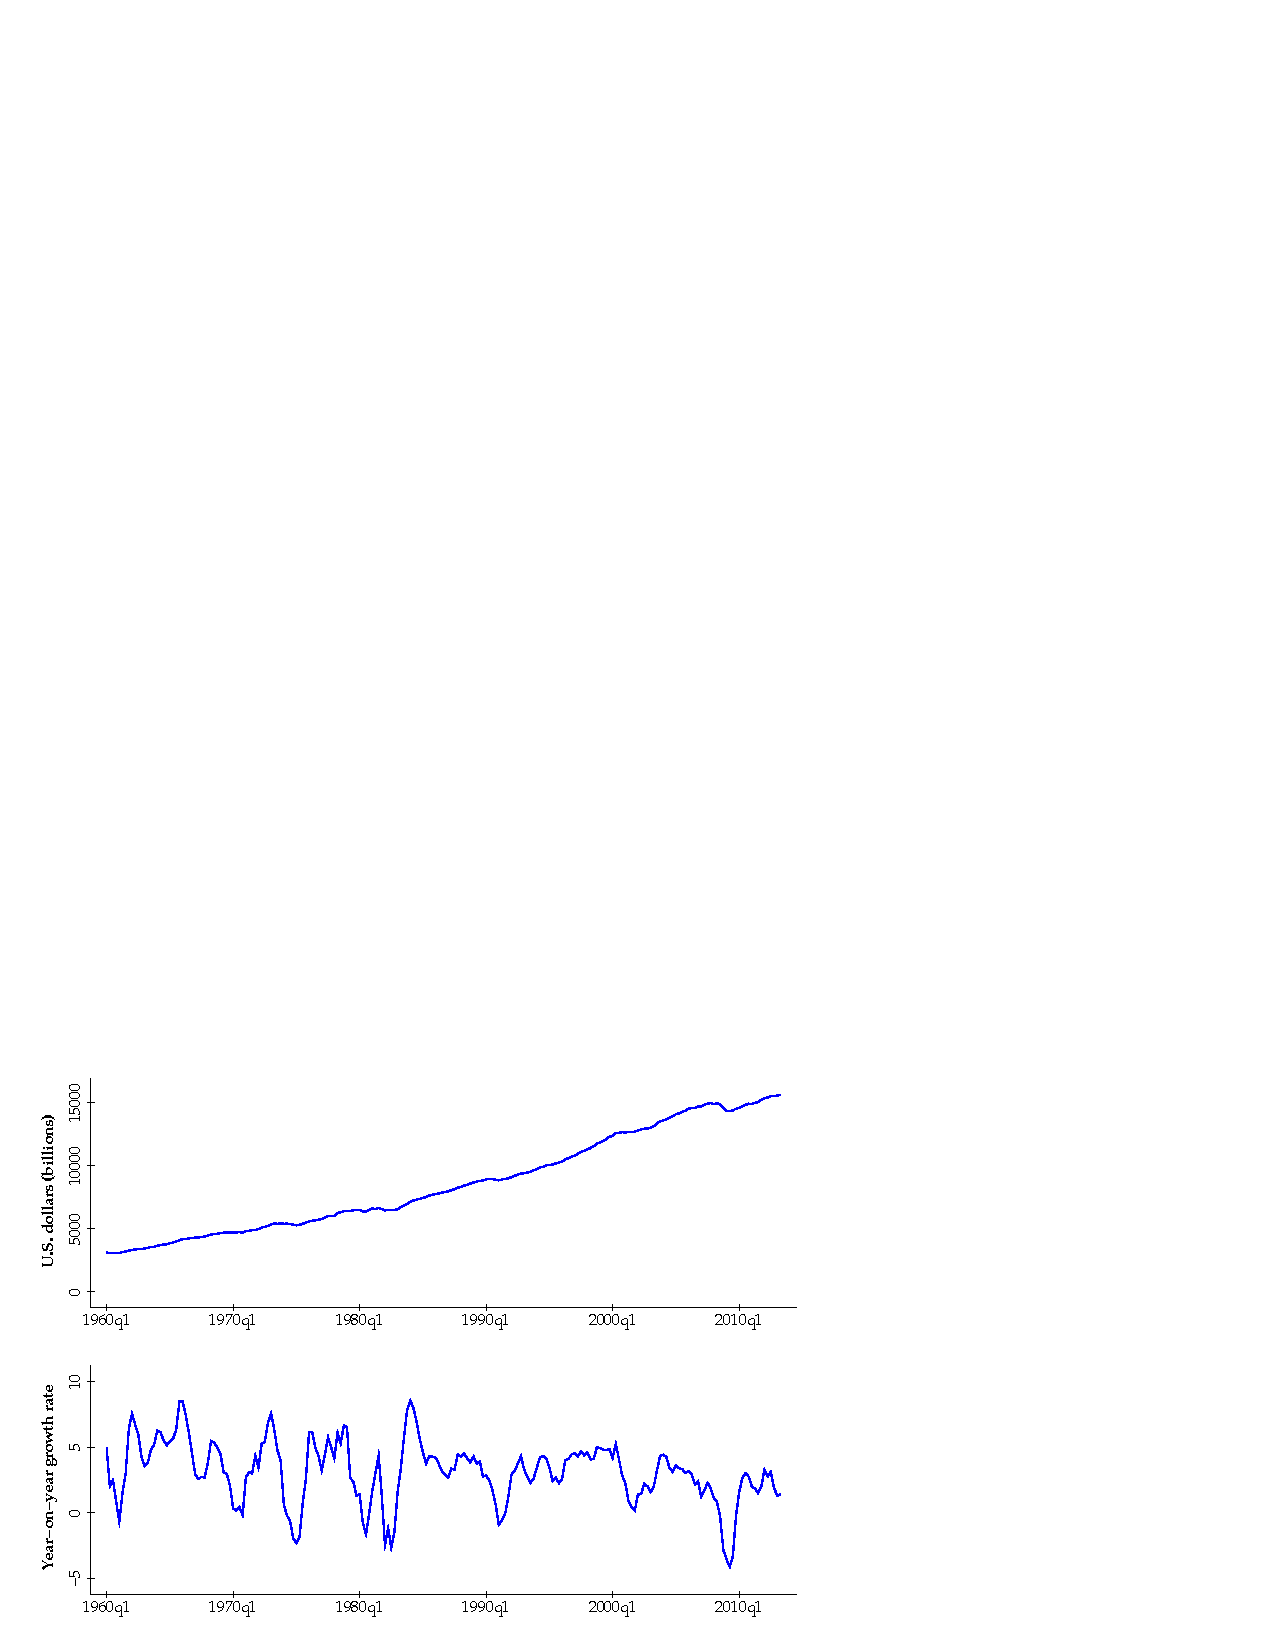
\includegraphics[width=0.8\textwidth]{Figures/us_gdp.pdf}
\end{figure}

The \href{http://www.nber.org/cycles/main.html}{National Bureau of Economic Research},
which dates business cycles in the US,
defines a recession \index{recession} as ``a significant decline
in economic activity spread across the economy,
lasting more than a few months, normally visible in real GDP,
real income, employment, industrial production,
and wholesale-retail sales.''
Using subjective methods, they identify dates of peaks and troughs.
Less formally, many people use the rule of thumb
that a recession consists of two consecutive quarters
in which GDP has fallen.
The year-on-year growth rates in the figure don't coincide exactly
with this definition, but you can see the eight official NBER
recessions since 1960 as sharp downward spikes in GDP growth.


\section{Expenditure components}

Burns and Mitchell refer to fluctuations in
``many economic activities.''
Among these activities are the expenditure
components of GDP.
Are their fluctuations similar to those of GDP?
On the whole, the components, particularly consumption and investment,
move up and down together, but the magnitudes differ enormously.
\href{http://research.stlouisfed.org/fred2/series/PCECC96?cid=110}{Consumption}
currently accounts for about 70 percent of US GDP;
as you might expect, its fluctuations are similar (see Figure \ref{fig:gcall}).
The correlation of year-on-year growth rates in consumption (total)
and GDP is 0.84.\index{gross domestic product (GDP)!real GDP|)}

Table \ref{tab:cycleprops} shows us that consumption's components ---
services, nondurable goods, and durable goods --- also vary with GDP,
but their correlations and (esp) volatilities differ somewhat.
Consumption of nondurables and services
is less volatile than GDP, in the sense that
the standard deviation of its growth rate is smaller.
Consumption of durables is far more
volatile %(in the sense that its standard deviation is larger)
than consumption of nondurables and services.
You might think of specific products and industries that reflect
the same phenomenon.
Why do you think cars and refrigerators
are more volatile than haircuts and medical care?

\begin{table}[h!]
\centering
\caption{Properties of business cycles.}
\label{tab:cycleprops}
\begin{tabular*}{0.8\textwidth}{l@{\extracolsep{\fill}}ccc}
\toprule
        &  Std Dev (\%)  &  Corr w/ GDP  \\
\midrule
GDP     &      2.19          &    1.00      \\
Consumption:  total      &  1.75  &  0.84   \\
Consumption:  services   &  1.22  &  0.63   \\
Consumption:  nondurable &  1.65  &  0.75   \\
Consumption:  durables   &  6.29  &  0.76   \\
Investment:  total       &  6.64  &  0.86   \\
Investment:  structures  &  7.85  &  0.46   \\
Investment:  equipment   &  7.35  &  0.81   \\
Investment:  housing     &  13.05\phantom{1} &  0.60   \\
Employment               &  1.77  &  0.76   \\
S\&P 500 Index           &  14.98\phantom{1}  &  0.36   \\
\bottomrule
\addlinespace
\end{tabular*}
\begin{minipage}{0.8\textwidth}
\footnotesize{Numbers refer to year-on-year growth rates computed from quarterly US data.}
\end{minipage}
\end{table}

\begin{figure}[h!]
    \caption{Fluctuations in consumption, investment, and GDP.}
    \label{fig:gcall}%
    \centering
    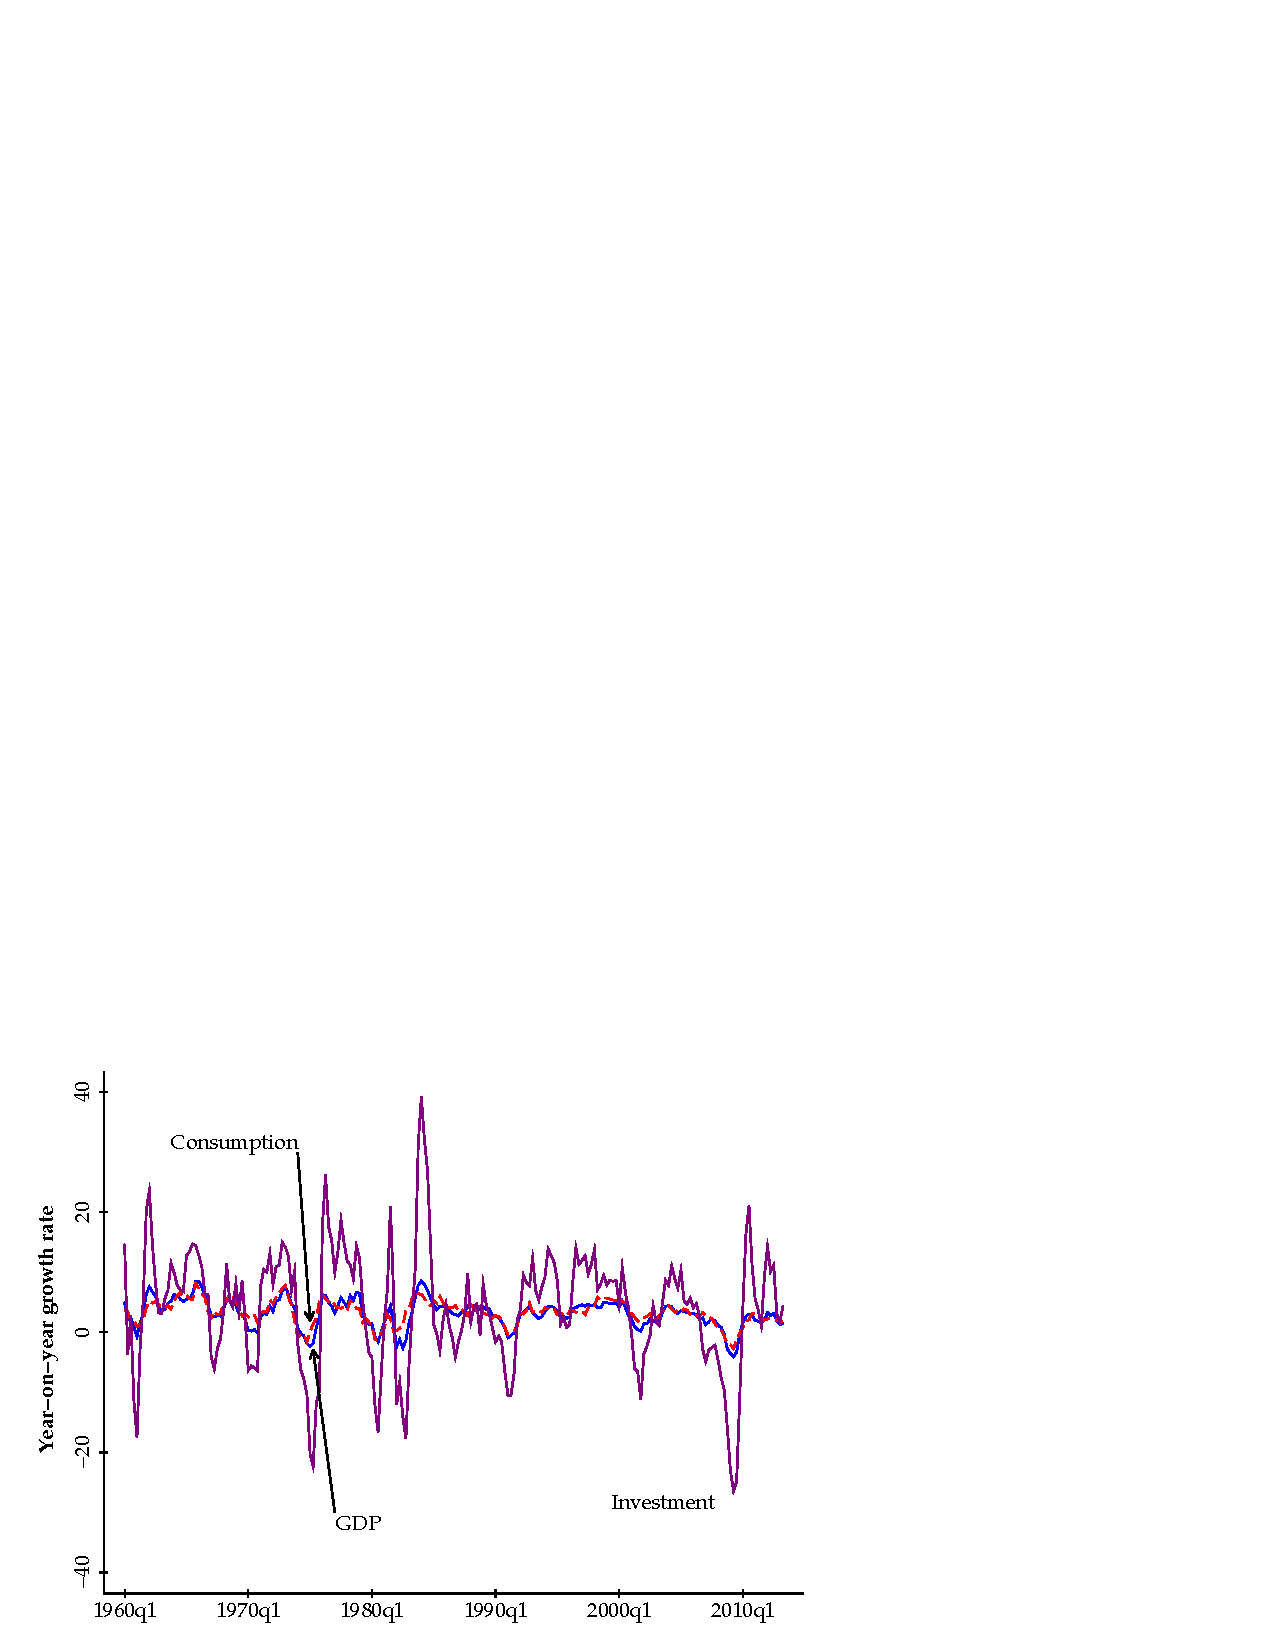
\includegraphics[width=0.8\textwidth]{Figures/us_inv_cons_gdp.pdf}
\end{figure}

\href{http://research.stlouisfed.org/fred2/series/GPDIC96?cid=112}{Investment}
also moves up and down with output
and is substantially more volatile (see Figure \ref{fig:gcall}).
As a rule of thumb, a one-percent increase in GDP is associated with
about a three-percent increase in total investment.
(We're looking at the ratio of standard deviations here,
and the high correlation of the two series.)
Table \ref{tab:cycleprops}
shows that the major components of investment --- structures, equipment,
and residential housing --- are highly correlated with,
and more volatile than, GDP.


When we turn to \index{cyclical indicators}
business-cycle indicators, we'll see that
many of them are more detailed measures of
some aspect of consumption or investment.
Consumption is important because it accounts for most of GDP.
Investment is important because it is highly responsive
to changes in economic conditions.


\section{Labor and capital markets move with the cycle}

Labor markets also move with the business cycle;
indeed, it's the way in which business cycles make themselves
known to us most directly.
Figure~\ref{fig:labor} shows us how fluctuations in
\href{http://research.stlouisfed.org/fred2/series/PAYEMS}{employment}
covary with GDP.
Note that employment growth is generally less than GDP growth;
the difference reflects an increase in output per worker --- a good thing, to be sure!
You can see in the figure that the ups and downs in employment
typically lag those in GDP by a little --- a quarter or two.
The current expansion is an extreme case, with
GDP rebounding well before employment,
but the general pattern is not unusual.

\begin{figure}[h!]
\caption{Fluctuations in employment and GDP.}
    \label{fig:labor}%
    \centering
    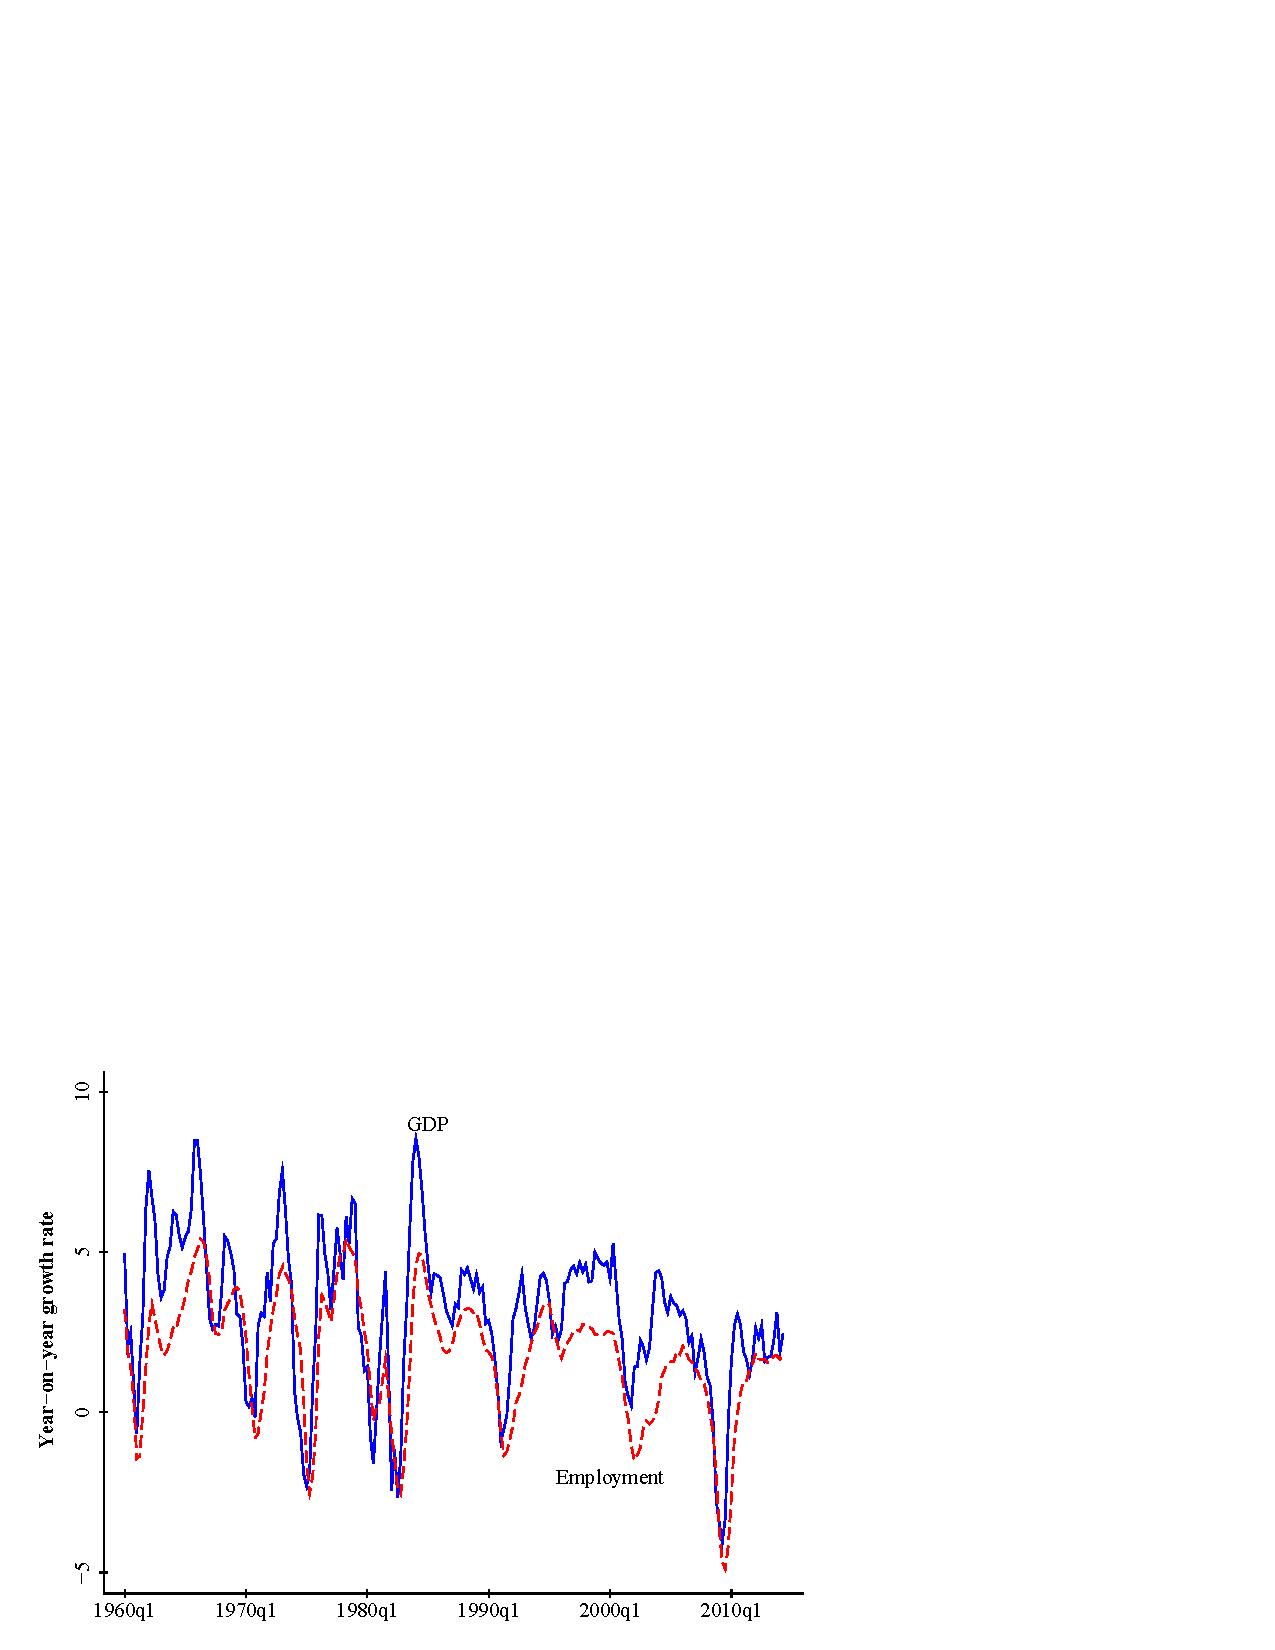
\includegraphics[width=0.8\textwidth]{Figures/us_emp_gdp.pdf}
\end{figure}

\begin{figure}[h!]
    \caption{Fluctuations in asset prices and GDP.}
    \label{fig:stock}%
    \centering
    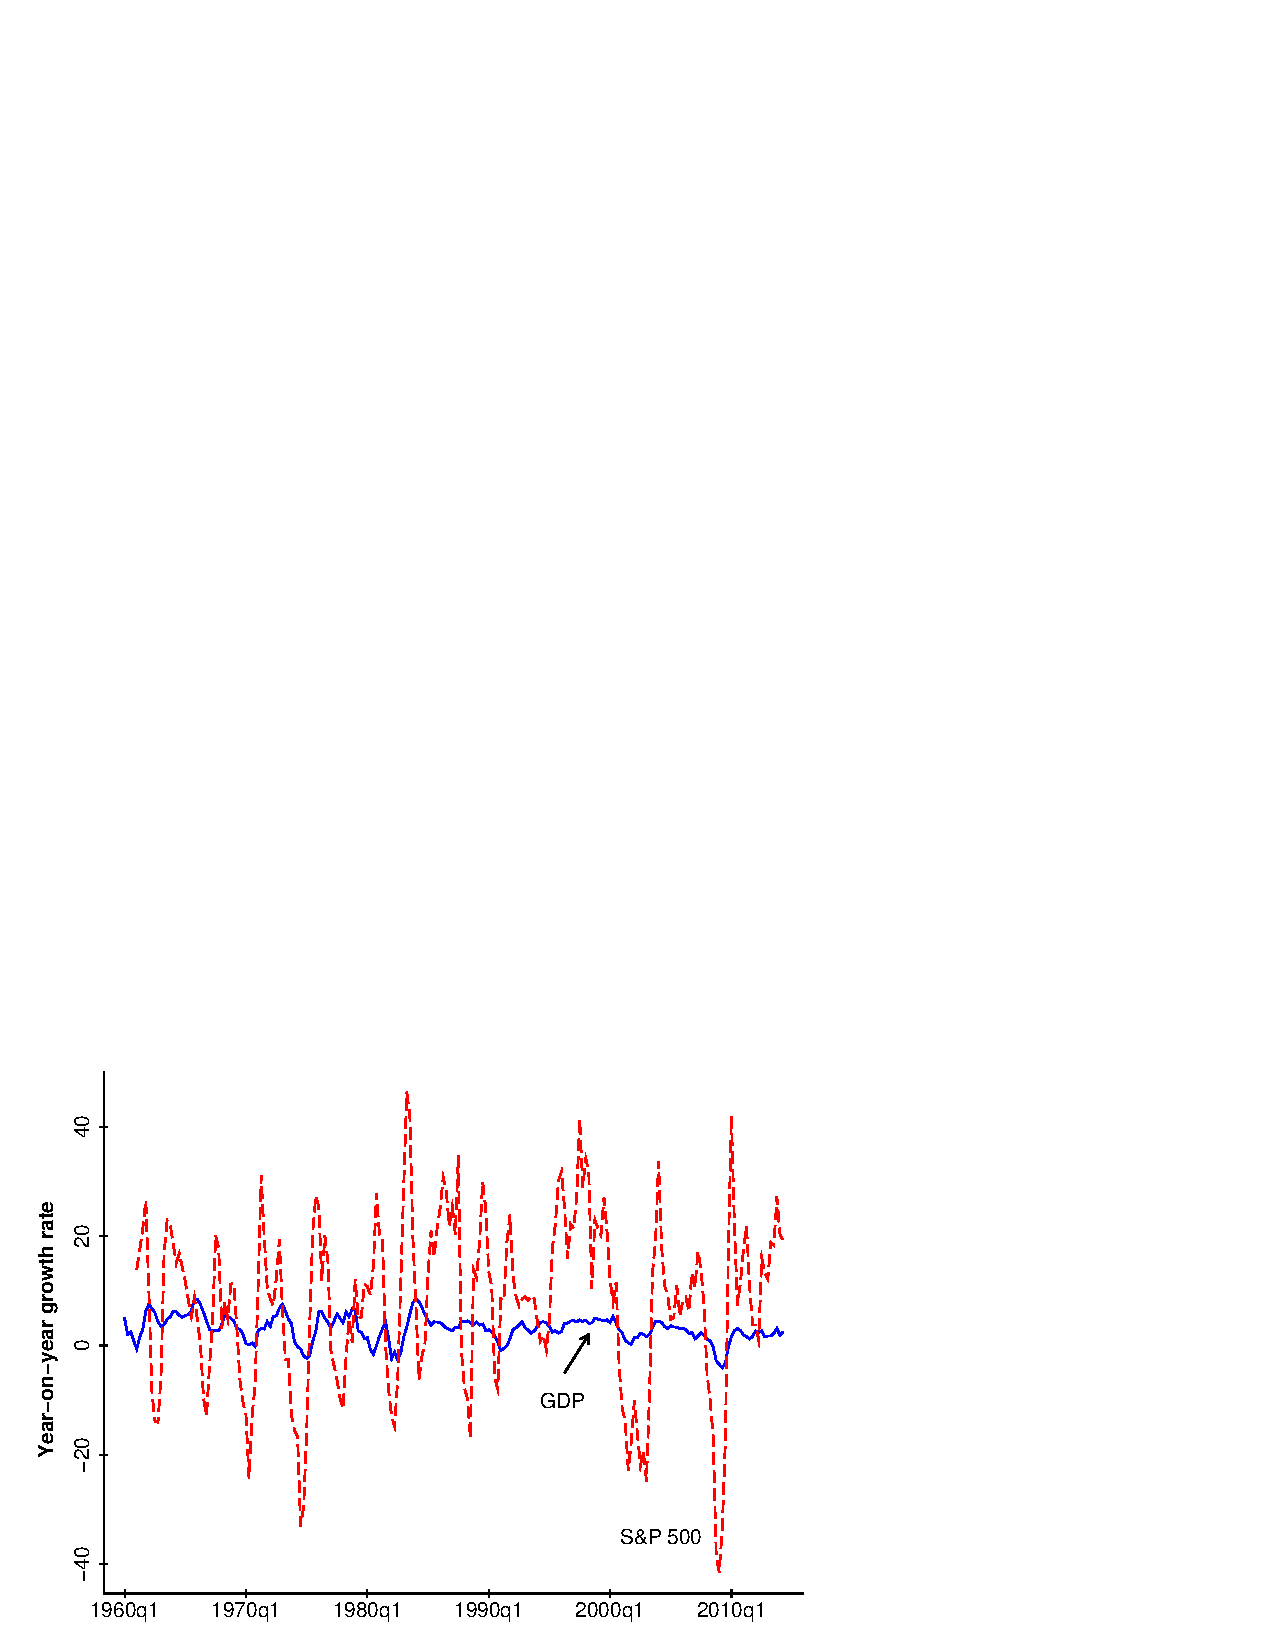
\includegraphics[width=0.8\textwidth]{Figures/us_gdp_sp500.pdf}
\end{figure}

Financial (capital) markets move with the business cycle, as well. Figure \ref{fig:stock} plots the growth rate of real GDP\index{gross domestic product (GDP)!real GDP} against versus the yearly growth rate of the \href{http://research.stlouisfed.org/fred2/series/SP500}{S\&P 500 index}. Notice that aggregate stock prices are extremely volatile, with a standard deviation about eight times larger than GDP. Moreover, aggregate stock prices and GDP are positively correlated (0.36). This suggests that good news about the economy is good news for stock prices.
It's hard to see in Figure \ref{fig:stock},
but we'll see later that stock prices lead GDP;
the correlation of stock prices with GDP two quarters later is above 0.5. Financial
measures often lead economic activity. Another example is the yield \index{bond!bond yield}
 curve (the difference
between long-term and short-term interest rates),
which tends to flatten or invert ahead of business downturns.
We'll look at this more closely when we turn to indicators.


Labor markets and asset prices are
both sources of useful indicators of economic activity.
We'll see more of each shortly.


\section*{Executive summary}

\setlength{\leftmargini}{.5\oldleftmargini}
\begin{enumerate}
\item Economies do not grow smoothly; they exhibit lots of
short-term volatility.

\item Spending on investment goods (by firms)
and consumer durables (by households) are more volatile
 than output as a whole.
 Household spending on nondurable goods and services
 is less volatile than output.

\item Most variables are procyclical\index{business cycle!procyclical}; that is, they move up and down with GDP.
Examples include consumption, investment, employment, and the stock market.
\end{enumerate}
\setlength{\leftmargini}{\oldleftmargini}

\section*{Review questions}

\setlength{\leftmargini}{.5\oldleftmargini}
\begin{enumerate}
\item Statistics.  What statistic would you use to show that two economic series
move up and down together?

Answer.  The correlation between them.
Table \ref{tab:cycleprops}, for example, includes the correlations
of year-on-year growth rates of GDP and several expenditure components.
The correlations in most cases are above 0.8, indicating they do indeed
mostly move up and down together.

\item More statistics.  What statistic would you use
 to show that one series is more ``volatile''
than another.

Answer.  The standard deviation.
In the same table, we saw that investment is more volatile than consumption
in the sense that its standard deviation is about three times higher.

\item Do it yourself.  Reproduce Figure \ref{fig:labor} in FRED.
The variables are real GDP (FRED code GDPC1) and nonfarm employment
(PAYEMS).
\end{enumerate}
\setlength{\leftmargini}{\oldleftmargini}

\section*{If you're looking for more}

These basic features of business cycles \index{business cycle|)}
 are covered in most
macroeconomics textbooks.
A reasonably good overview is Finn Kydland and Edward Prescott,
``\href{http://www.minneapolisfed.org/publications_papers/pub_display.cfm?id=225}
{Real facts and a monetary myth}.''

\section*{Data used in this chapter}

\begin{table}[H]
\centering
\caption{Data table.}
\begin{tabular*}{0.8\textwidth}{l@{\extracolsep{\fill}}l}
\toprule
Variable & Source\\
\midrule
GDP                            &GDPC1\\
Consumption                    &PCECC96 \\
\hspace{0.2in}Services        &PCESVC96\\
\hspace{0.2in}Durables        &PCDGCC96\\
\hspace{0.2in}Nondurables    &PCNDGC96\\
Investment                    &GPDIC96\\
\hspace{0.2in}Nonresidential &PNFIC96\\
\hspace{0.4in}Equipment        &NRIPDC96\\
\hspace{0.2in}Housing        &PRFIC96\\
Employment                    &PAYEMS\\
S\&P500                     &SP500\\
10yr Treasury yield \index{bond!bond yield}
            &GS10\\
2yr Treasury yield \index{bond!bond yield}
            &GS2\\
Federal funds rate            &FEDFUNDS\\
\bottomrule
\addlinespace
\end{tabular*}
\begin{minipage}{0.8\textwidth}
\footnotesize{To retrieve the data online, add the identifier from the source column to \url{http://research.stlouisfed.org/fred2/series/}.  For example, to retrieve nonfarm employment, point your browser to \url{http://research.stlouisfed.org/fred2/series/PAYEMS}}
\end{minipage}
\end{table}
